 \documentclass{llncs}
 \usepackage{amsmath}
\usepackage{amssymb}
\usepackage{graphicx}
\usepackage{enumerate}
\usepackage{url}

\newcommand{\tup}[1]{\langle #1 \rangle}
\newcommand{\vvec}[1]{\mathbf{#1}}
\newcommand{\join}{\bowtie}
\newcommand{\R}{\mathcal{R}}
\newcommand{\Q}{\mathcal{Q}}
\newcommand{\qrule}{:\!\!-}
\newcommand{\mcdsat}{\textsc{McdSat}}
\newcommand{\minicon}{{MiniCon}}
\newcommand{\Omit}[1]{}

% flights
\newcommand{\flight}{\text{\it flight}}
\newcommand{\UScity}{\text{\it uscity}}
\newcommand{\national}{\text{\it national}}
\newcommand{\oneway}{\text{\it one-way}}
\newcommand{\onestop}{\text{\it one-stop}}
\newcommand{\flightPA}{\text{\it flight-to-pa}}
\newcommand{\onestopPA}{\text{\it onestop-to-pa}}
\newcommand{\fromNY}{\text{\it from-ny}}
\newcommand{\PA}{\text{PA}}
\newcommand{\NY}{\text{NY}}
\newcommand{\AL}{\text{AL}}

\begin{document}
\allowdisplaybreaks
\title{SatWins: A Sat-based tool to Optimal Instantiations of Abstract Workflows}
\author{Daniel Izquierdo \and Mar\'{\i}a-Esther Vidal \and Blai Bonet}
\institute{Departamento de Computaci\'on \\
           Universidad Sim\'on Bol\'{\i}var \\
           Caracas 89000, Venezuela \\
           \url{{idaniel,mvidal,bonet}@ldc.usb.ve}}
\maketitle

\begin{abstract}
We present SatWins a system to efficiently solve the abstract workflow
instantiation problem that is firmly grounded on logic.
SatWins adopts the Local-As-View approach in which
the functionality of concrete services is described using views
of abstract services, the quality of an instantiation as an
overall utility function that combines the different QoS parameters,
and the abstract workflows as conjunctive queries on abstract services.
We discuss the encoding of the workflow instantiation problem as a logical theory whose models
are in correspondence with the instantiations of the workflow,
and the best ranked models are in correspondence with the
optimal instantiations of the workflow. We demonstrate how by exploiting known properties of logical theories in 
d-DNNF format, SatWins provides an efficient and scalable solution
to the workflow instantiation problem. 
\end{abstract}

\section{Introduction}
Emerging technologies support the basis for the wealth of available Web resources, as well as current users' tendency to rely more on automatic methods for handling existing Web resources or services composed in complex workflows. The execution of an abstract workflow involves the instantiation
of the abstract services into concrete services that meet the workflow
functional and non-functional requirements. This instantiation
process can be seen as a search for a target instantiation on
the combinatorial space of all valid instantiations.
Thus, one is interested in efficient techniques for performing
this search that are able to scale up as the number of concrete
services or the complexity of the workflow increases. We call the problem of instantiating a given abstract workflow with concrete services, from a given pool of concrete services,
such that certain QoS demands are meet, the Workflow Instantiation
Problem (WIP). 

In this paper, we describe SatWins a system that considers
 a restricted version of WIP that adopts
the Local-As-View (LAV) approach \cite{levy:bucket} to specify the semantics of the concrete services as views of abstract services; this representation is similar to the
one that is semi-automatically generated for the DEIMOS system
\cite{AmbiteISWC09}. Additionally,  abstract workflows correspond  to conjunctive
queries on the abstract services, and  the quality
of an instantiation is an overall utility function that combines the
different QoS parameters of the selected concrete services.
In this version of WIP, the rules that define workflows (conjunctive queries)
and concrete services (views) are created in a way that all the 
functional restrictions on pre- and post-conditions of services
and their combinations are satisfied, and the QoS measures are
represented by annotating each concrete service description with
a real number that represents the overall QoS utility of the service.

In addition to providing a novel approach to describe the WIP problem, SATWins is able to  efficiently identify an abstract workflow's instantiations. 
Given a WIP, a logical theory is constructed such that each model of
the theory encodes a valid instantiation, and thus all valid instantiations
are obtained by enumerating all models of the theory. This enumeration
can be efficiently performed if the logical theory is in a certain 
normal form called deterministic and decomposable negation normal
form (d-DNNF) \cite{darwiche:d-dnnfs}. Thus, the approach consists in
transforming (called compiling in the field of knowledge compilation)
the logical theory into d-DNNF format for enumerating its models efficiently; also, the  enumeration  of
the best ranked models can also be performed efficiently on a theory in d-DNNF and
the complexity is independent of the utility function used to rank the optimal instantiation.

In this demonstration, we  attempt to show the following key aspects of the approach implemented by SATWins. We will use a real-world example based on a simple flight-information system.
\begin{itemize}
\item We show the expressiveness of representing concrete services as views on abstract services.
\item We demonstrate the performance of the proposed techniques by computing the optimal instantiation of a given WIP in terms of different utility functions.  
\item We show the scalability of our solution by demonstrating how SATWins is able to enumerate realistic instances of the problem in less than one second.
\end{itemize}  
 
\section{SatWins Architecture}
 The SatWins architecture  is comprised of a Catalog of service descriptions,
the Encoder, the compiler c2d, the best model Finder, and the Decoder.
Figure~\ref{fig:architecture} depicts the overall architecture of the system.
In this framework, an instance of the Workflow Instantiation Problem is defined as an
abstract workflow represented by a conjunctive query on abstract services which
is given as input together with a set of concrete services defined by views
of abstract services. 

\begin{figure}[t]
\centering
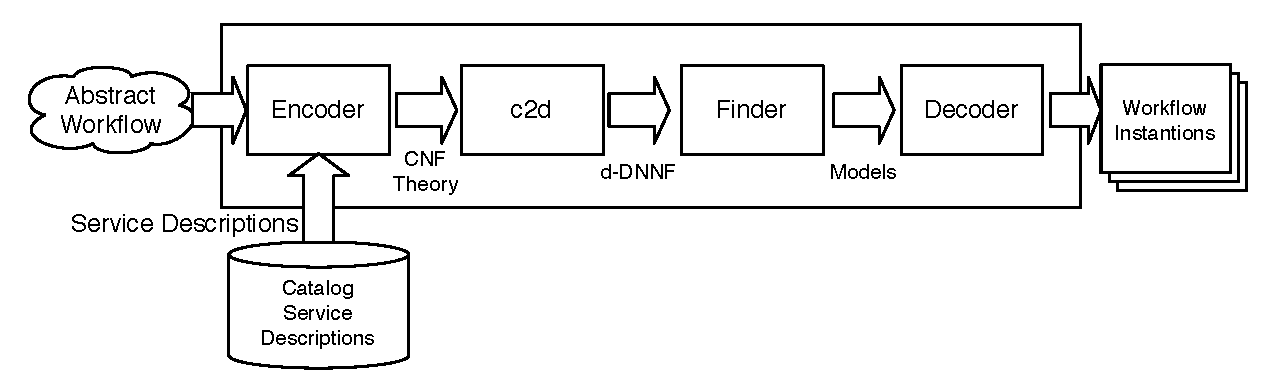
\includegraphics[width=.9\textwidth]{architecture}
\caption{The SatWins Architecture}
\label{fig:architecture}
\end{figure}

The Catalog is populated with descriptions of abstract and concrete services;
each service is described in terms of input and output attributes, and annotated
with a real value that represents the QoS utility of the service.
The description of the concrete services, that are defined as views of abstract
services, can be generated semi- or automatically using tools such as the DEIMOS
system \cite{AmbiteISWC09}. 

An input instance of WIP is encoded as a CNF theory whose models correspond to
the instantiations of the workflow by the Encoder. 
The compiler c2d, an off-the-shelf
component, compiles the CNF formula into d-DNNF.
The Encoder translates the WIP instances into CNF theories, that are then converted
into d-DNNF using c2d. The Finder computes a best model given the QoS parameters
in linear time in the size of the resulting d-DNNF. It is important to remark
that the compilation process needs to be performed only once as it does not
depend on the value of the QoS parameters. Thus, even if the compilation happens
to be costly in terms of time, this cost can be amortized since the resulting
d-DNNF can be used to find best instantiations with respect to multiple values
of the QoS parameters.
Finally, the Decoder translates the best model returned by the Finder into
a workflow instantiation that solves the WIP.

Given a CNF that encodes a WIP, its d-DNNF is a compact representation of
all the workflow instantiations. That is, one can generate in a backtrack-free
manner all the instantiations of the workflow. If the user is interested in
a best instantiation given the QoS parameters, then it can be computed in
linear time in the size of the d-DNNF. If the user is interested in the 
all the best instantiations, these can be computed in linear time in the
number of them. Finally, if the user is interested in all instantiations,
these can be also computed in linear time in the number of them.
In the latter two cases, if such number is exponential (in the size of the
input), the enumeration of the instantiations is also exponential but
this complexity is intrinsic to the problem and thus cannot be avoided.
Figure \~ref{fig:snapshot} shows a snapshot of an input instance of WIP and the functionality of SatWins. 

\begin{figure}[t]
\centering
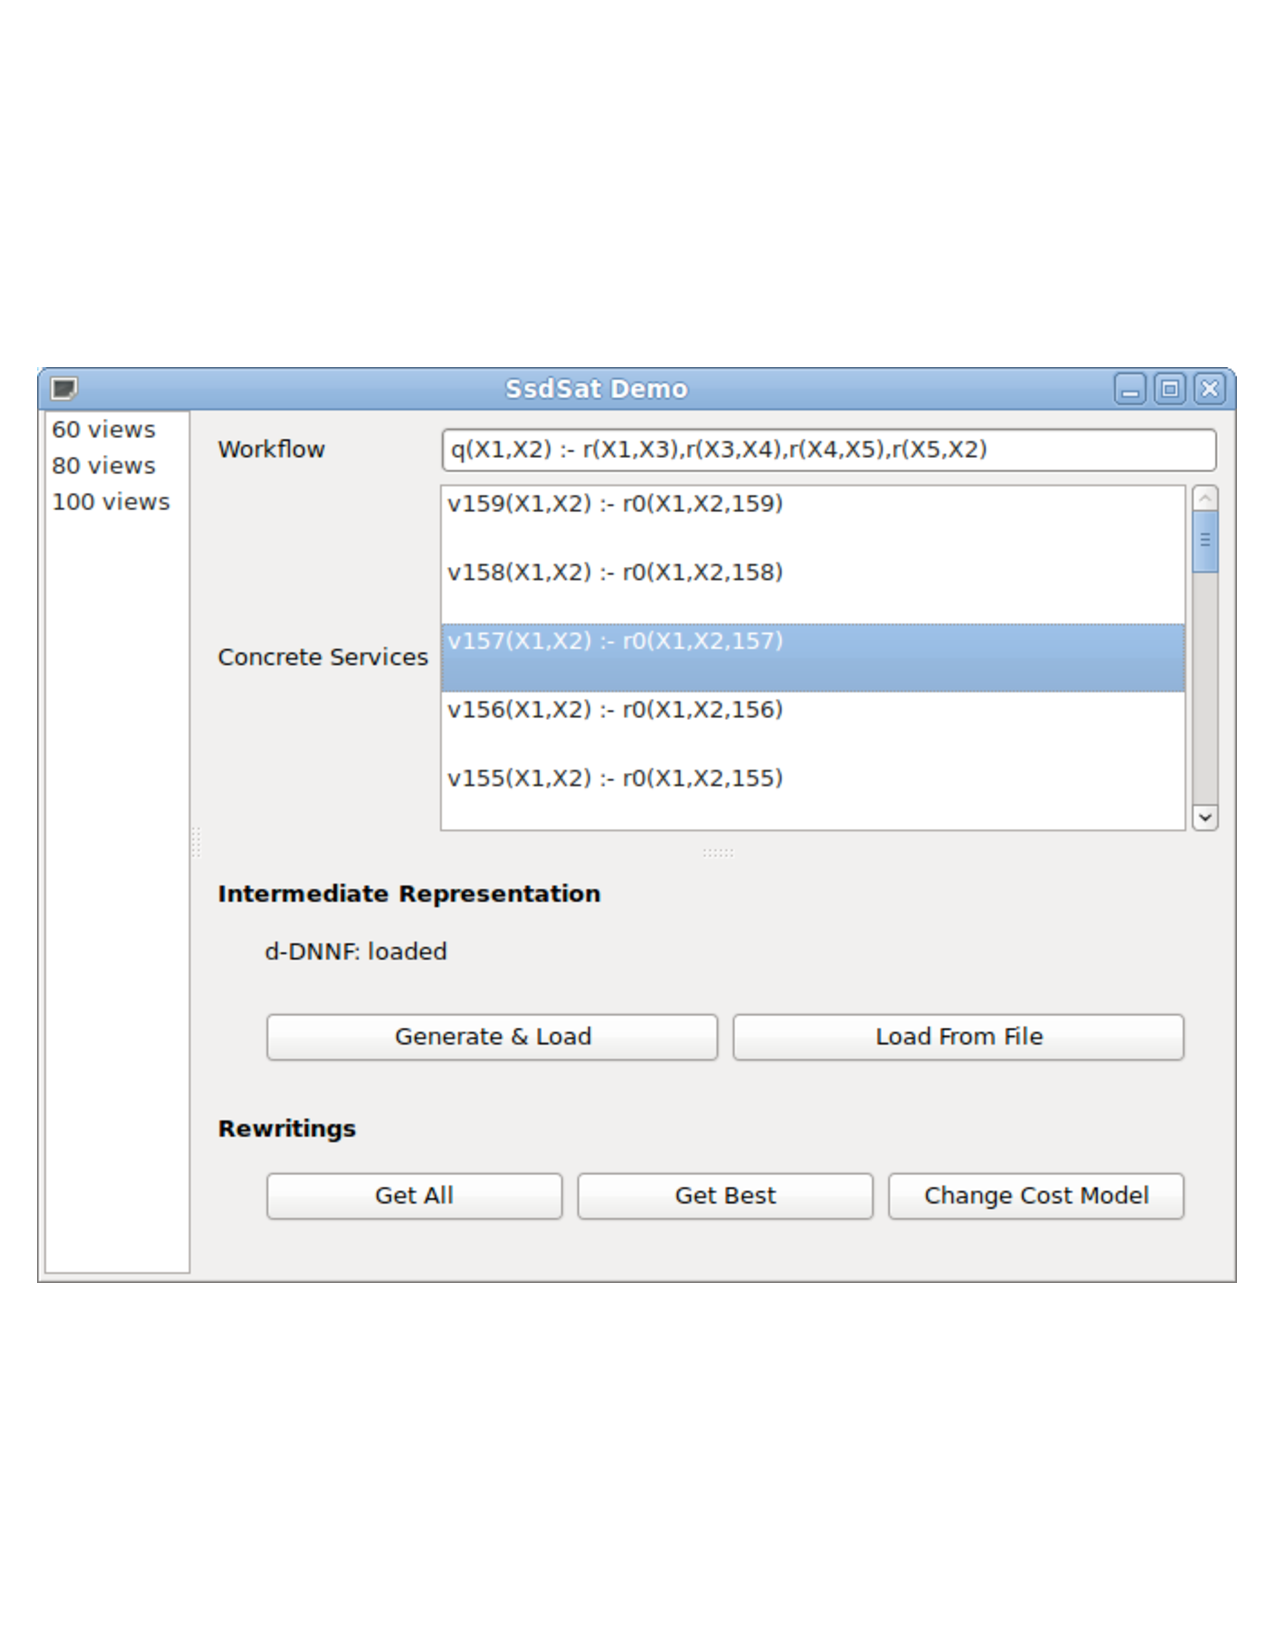
\includegraphics[height=30mm,width=.7\textwidth]{demo}
\caption{A snapshot of the SatWins interface}
\label{fig:snapshot}
\end{figure}

\section{Demonstration Use Cases}
In this demonstration, we will go through the different steps of the proposed approach.
We illustrate our approach on  a simple flight-information system which contains information
about flights between cities and information about which cities are in
the US. Such a system can be described using LAV with the two abstract
services $\flight(x,y)$ and $\UScity(x)$. The former relates two cities
$x$ and $y$ if there is a direct flight between them, and the latter tells
whether $x$ is a US city or not. We also consider different sets of concrete services; functionality, complexity and size will be changed during the demonstration to show
the expressiveness, performance and scalability of our approach. An example of some of the concrete services to be used is as follows:
\begin{enumerate}[--]
\item $\national(x,y)$ relates two US cities that are connected by a direct flight,
\item $\oneway(x,y)$ relates two cities that are connected by a one-way flight,
\item $\onestop(x,y)$ relates two cities that are connected by a one-stop flight,
\item $\flightPA(x)$ tells if there is a direct flight from $x$ to Paris,
\item $\onestopPA(x,y)$ relates $x$ and $y$ if there is a flight from $x$ to Paris
      with a stop at $y$, and
\item $\fromNY(x)$ tells if there is a flight from New York into $x$.
\end{enumerate}
The descriptions of these concrete services using the abstract services:
\begin{alignat*}{1}
\national(x,y)\   &\qrule\ \flight(x,y),\,\UScity(x),\,\UScity(y)\,. \\
\oneway(x,y)\     &\qrule\ \flight(x,y)\,. \\
\onestop(x,z)\    &\qrule\ \flight(x,y),\,\flight(y,z)\,. \\
\flightPA(x)\     &\qrule\ \flight(x,\PA)\,. \\
\onestopPA(x,y)\  &\qrule\ \flight(x,y),\,\flight(y,\PA)\,. \\
\fromNY(x)\       &\qrule\ \flight(\NY,x)\,.
\end{alignat*}

In addition, the following abstract workflow to retrieve
the one-stop round-trip flights from US cities to any city in the world, such that
flights can stop at any city, is represented as a conjunctive query on the abstract services as follows: 
\[ W(x,w,y,z) \qrule \UScity(x),\,\flight(x,w),\,\flight(w,y),\,\flight(y,z),\,\flight(z,x)\,. \]

Any instantiation of the abstract services in terms of
concrete services is a valid implementation of the workflow or concrete service compositions.
For example, the following composition corresponds to one such implementation.
\[ I(x,w,y,z)\ \qrule\ \national(x,w),\,\flightPA(w),\,\oneway(\PA,z),\,\national(z,x)\,. \]
However, the following composition is not valid.
\begin{alignat*}{1}
I'(x,w,y,z)\  \qrule\ &\national(x,y),\,\flightPA(y),\,\fromNY(z),\,\national(z,x)\,. \\
\end{alignat*}

Using this domain, we will demonstrate the following scenarios:
\begin{itemize}
\item To show the scalability of the proposed approach, we use the behavior of
SATWins in three different benchmarks. In all the cases, we show time for
compilation, size of the  d-DNNF, and time to enumerate all the models as well
as the optimal one. We start with a benchmark of instances for workflows with 2
to 5 sub-goals and sets of 10 to 100 concrete services. Although the observed
time suggests a sub-exponential behavior, in any case, the results
show good performance. For instance, sets of 100
airlines with 5-stop flights can be compiled in 328 seconds; the size in disk of the d-DNNF is 3.4Mb;
the best model can be computed in 0.29 seconds, and the enumeration of all models in 0.47 seconds.
Then, in an attempt to induce an exponential growth in the compilation time, we add a second concrete service for each airline and we will show that SATWins behavior remains similar. Finally, we  involve concrete services with multiple sub-goals which are randomly generated.  The compilation time for these instances does not grow monotonically
since they are randomly generated. The same happens for the size of
the theories and the number of models. For example, the d-DNNF for 
a problem with 45 views each with 5 sub-goals is of size 5.1Mb and has
$1.26\times 10^8$ models. The time to find the best model for
this d-DNNF is 0.46 seconds while the time to enumerate all models
is about 17 hours.
\item To show the performance of the approach and reusability of existing d-DNNF, we will allow users to choose different utility metrics to compute the best solution.  We will show that the existing d-DNNF can be used to compute the best model with different utility functions, while the execution time remains the same for the different functions. 
\end{itemize}

\section{Conclusions}
In this demonstration, we will present a Local-As-View (LAV)-based approach \cite{levy:bucket} to WIP. We will show how by using simple conjunctive rules the functionality of concrete services and abstract workflows can be defined. In addition, we will show how a propositional-based approach can be used to represent instances of WIP and different scenarios where the performance and scalability of the technique will be observed by the users.  We will demonstrate that the approach can be applied to
real-sized workflow problems, while the whole approach is only possible
when the compilation of the CNF theory into d-DNNF format succeeds.
\bibliographystyle{abbrv}
\bibliography{ref}
 \end{document}
